\section{Samenwerking}
\todo{Dit moet naar het begin van het verslag}
Tijdens het ontwikkelen van de eerste versie van Canvas.HS is er samengewerkt volgens een paar vooraf geselecteerde methoden. Zo zijn er onderdelen van de Scrum projectmanagement methode gebruikt alsmede andere Agile methoden.

De samenwerking is goed verlopen. Daarbij was de duidelijke structuur van zowel het project– als de technische organisatie een belangrijk onderdeel. Er kon met deze structuur, naar gevoel van de projectgroep, efficiënt gewerkt worden. Er werd wekelijks twee of meer keer samengekomen om te werken aan het project.

\subsection{Project organisatie}
Er is gewerkt middels de scrum projectmangement methoden. Er is gewerkt met verschillende rollen en er zijn zogenaamde scrum en sprint besprekingen gehouden. Daarbij zijn elke keer opnieuw onder andere het project– en sprintbacklog samengesteld en bijgewerkt.

\paragraph{Rollen} Er is een verdeling van verantwoordelijkheden gemaakt. Naast de teamleden nam de opdrachtgever de rol van \emph{product owner} aan.
\begin{enumerate}
    \item \emph{J. van Doorn} had de taak van \emph{scrum master} en was verantwoordelijk voor het testen van de software.
    \item \emph{P.T. Jager} was notulist voor alle besprekingen en samen met Buit verantwoordelijk voor de Haskell code.
    \item \emph{L.J. Buit} was verantwoordelijk voor het protocol en samen met Jager verantwoordelijk voor de Haskell code.
    \item \emph{M.J. Roo} was samen met Scheepers verantwoordelijk voor de JavaScript code.
    \item \emph{M.J. Scheepers} was verantwoordelijk voor de gebruiksvriendelijkheid uiteindelijke API en samen met Roo verantwoordelijk voor de JavaScript code.
\end{enumerate}

\paragraph{Besprekingen} Elke samenkomst is er een kortdurende scrumbespreking gehouden. Na aanvang van het project zijn er ook een aantal sprint besprekingen gehouden. Deze sprint besprekingen kwamen altijd na het gesprek met de opdrachtgever. Er bleek al snel dat onze afgesproken sprint van twee werken wel erg kort was om elke twee weken dat er samengekomen werd een nieuwe lange sprintbespreking te houden. Dus er werd uiteindelijk voor gekozen om de besprekingen met de projectgroep te beperkingen tot de dagelijkse korte besprekingen.

Bij de dagelijkse besprekingen werd vaak op details in gegaan, hierbij werden ontwerp beslissingen vaak genomen tijdens deze besprekingen. De besprekingen duurde hierdoor soms wat lang en werden zittend gehouden.

\paragraph{Taken}
Regelmatig werd de lijst met taken bijgewerkt. Taken bestonden uit: projecttaken, als het bijhouden van de planning; ontwikkeltaken, als het oplossen van bugs en het schrijven van nieuwe features; schrijftaken en overige taken.

\begin{figure}[H]
\begin{center}
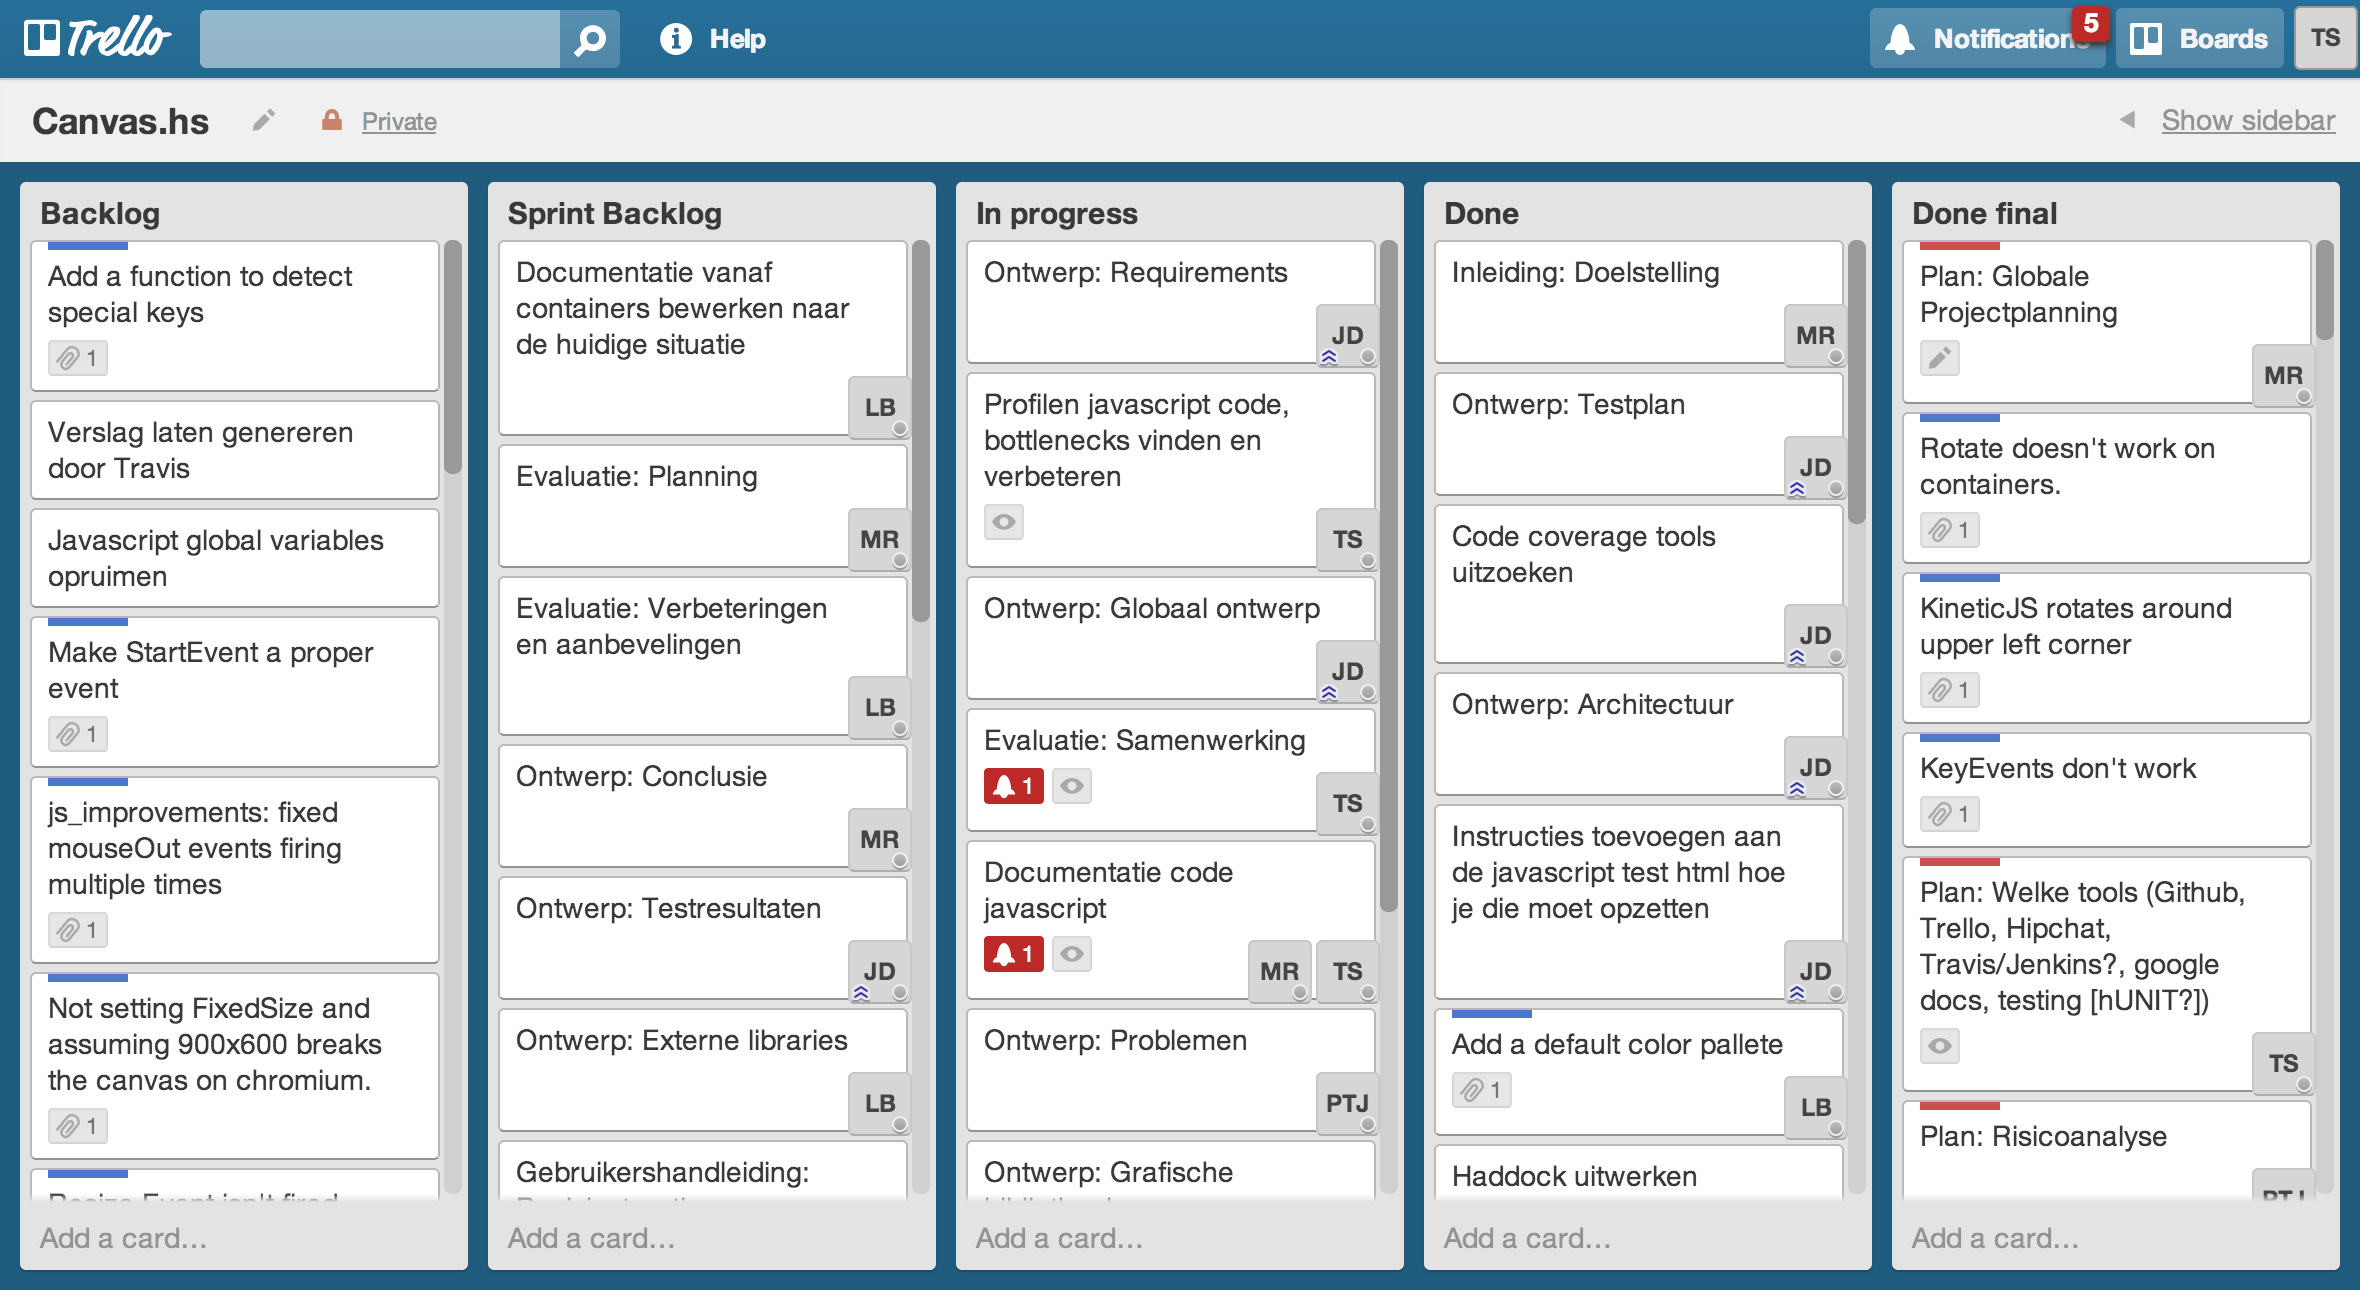
\includegraphics[keepaspectratio,width=\textwidth]{./images/trello.png}
\caption{Trello board}
\label{fig:trello}
\end{center}
\end{figure}

De lijst van ontwikkeltaken werd bijgehouden op het \emph{GitHub} platform. Deze taken werden daar ook wel Issues genoemd. Andere taken werden vervolgens bijgehouden op \emph{Trello}. Met deze applicatie kan een online takenbord gemaakt worden, zie \autoref{fig:trello}. De ontwikkeltaken werden middels synchronisatie ook op dit takenbord gezet. Door \emph{Trello} had elk lid van het project een goed inzicht in de taken die nog openstonden en reeds waren uitgevoerd.

\paragraph{Terugkoppeling naar de opdrachtgever} De opdrachtgever—binnen scrum ook \emph{product owner} genoemd—is twee wekelijks ge\"informeerd over de voortgang. De terugkoppeling die de opdrachtgever gaf werd besproken en verwerkt in de volgende versie van de library.

\paragraph{Verbeteringen} Er is nu gewerkt in een projectgroep zonder direct uren budget, mocht dit het geval zijn zouden de inschattingsmethoden en burndown chart uit de scrum methode kunnen worden gebruikt. Verder zouden de besprekingen zogenaamde \emph{stand-up meetings} kunnen worden waarbij iedereen staat en niet voor de computer zit. Hierdoor konden de dagelijkse besprekingen wellicht wat vlotter verlopen.

\subsection{Versiebeheer}
Bij het bouwen van software met een groep is het belangrijk dat een ontwikkelaar zich kan concentreren op de feature die hij aan het ontwikkelen is. Idealiter hoeft er geen rekening gehouden te worden met andere features die door anderen ontwikkeld worden. Er is dan ook gekozen om gebruik te maken van het gedistribueerde versiebeheer systeem \emph{Git} met een centraal repository op \emph{GitHub}.

Over het gebruik van deze software zijn afspraken gemaakt. Zo is er gebruik gemaakt van verschillende \emph{branches}. Als een bepaalde versie van de software op een bepaalde branch staat zegt dit iets over de status van die versie. Zo kan er begonnen worden aan een nieuwe feature vanaf de \inlinecode{dev} branch. En is een versie op de \inlinecode{master} branch klaar voor gebruik.

\paragraph{Feature branches en pull requests}
Bij aanvang van de ontwikkeling van een nieuwe feature werd er een nieuwe branch gemaakt vanaf de \inlinecode{dev} branch. Een voorbeeld hiervan is de \inlinecode{arcs} branch. In \autoref{sec:shapesext} staat beschreven hoe \inlinecode{Arc} shapes toegevoegd kunnen worden. Dit is dus gebeurd op een aparte branch die begonnen is vanaf de \inlinecode{dev} branch, zie \autoref{fig:pullrequest}. 

\begin{figure}
\begin{center}
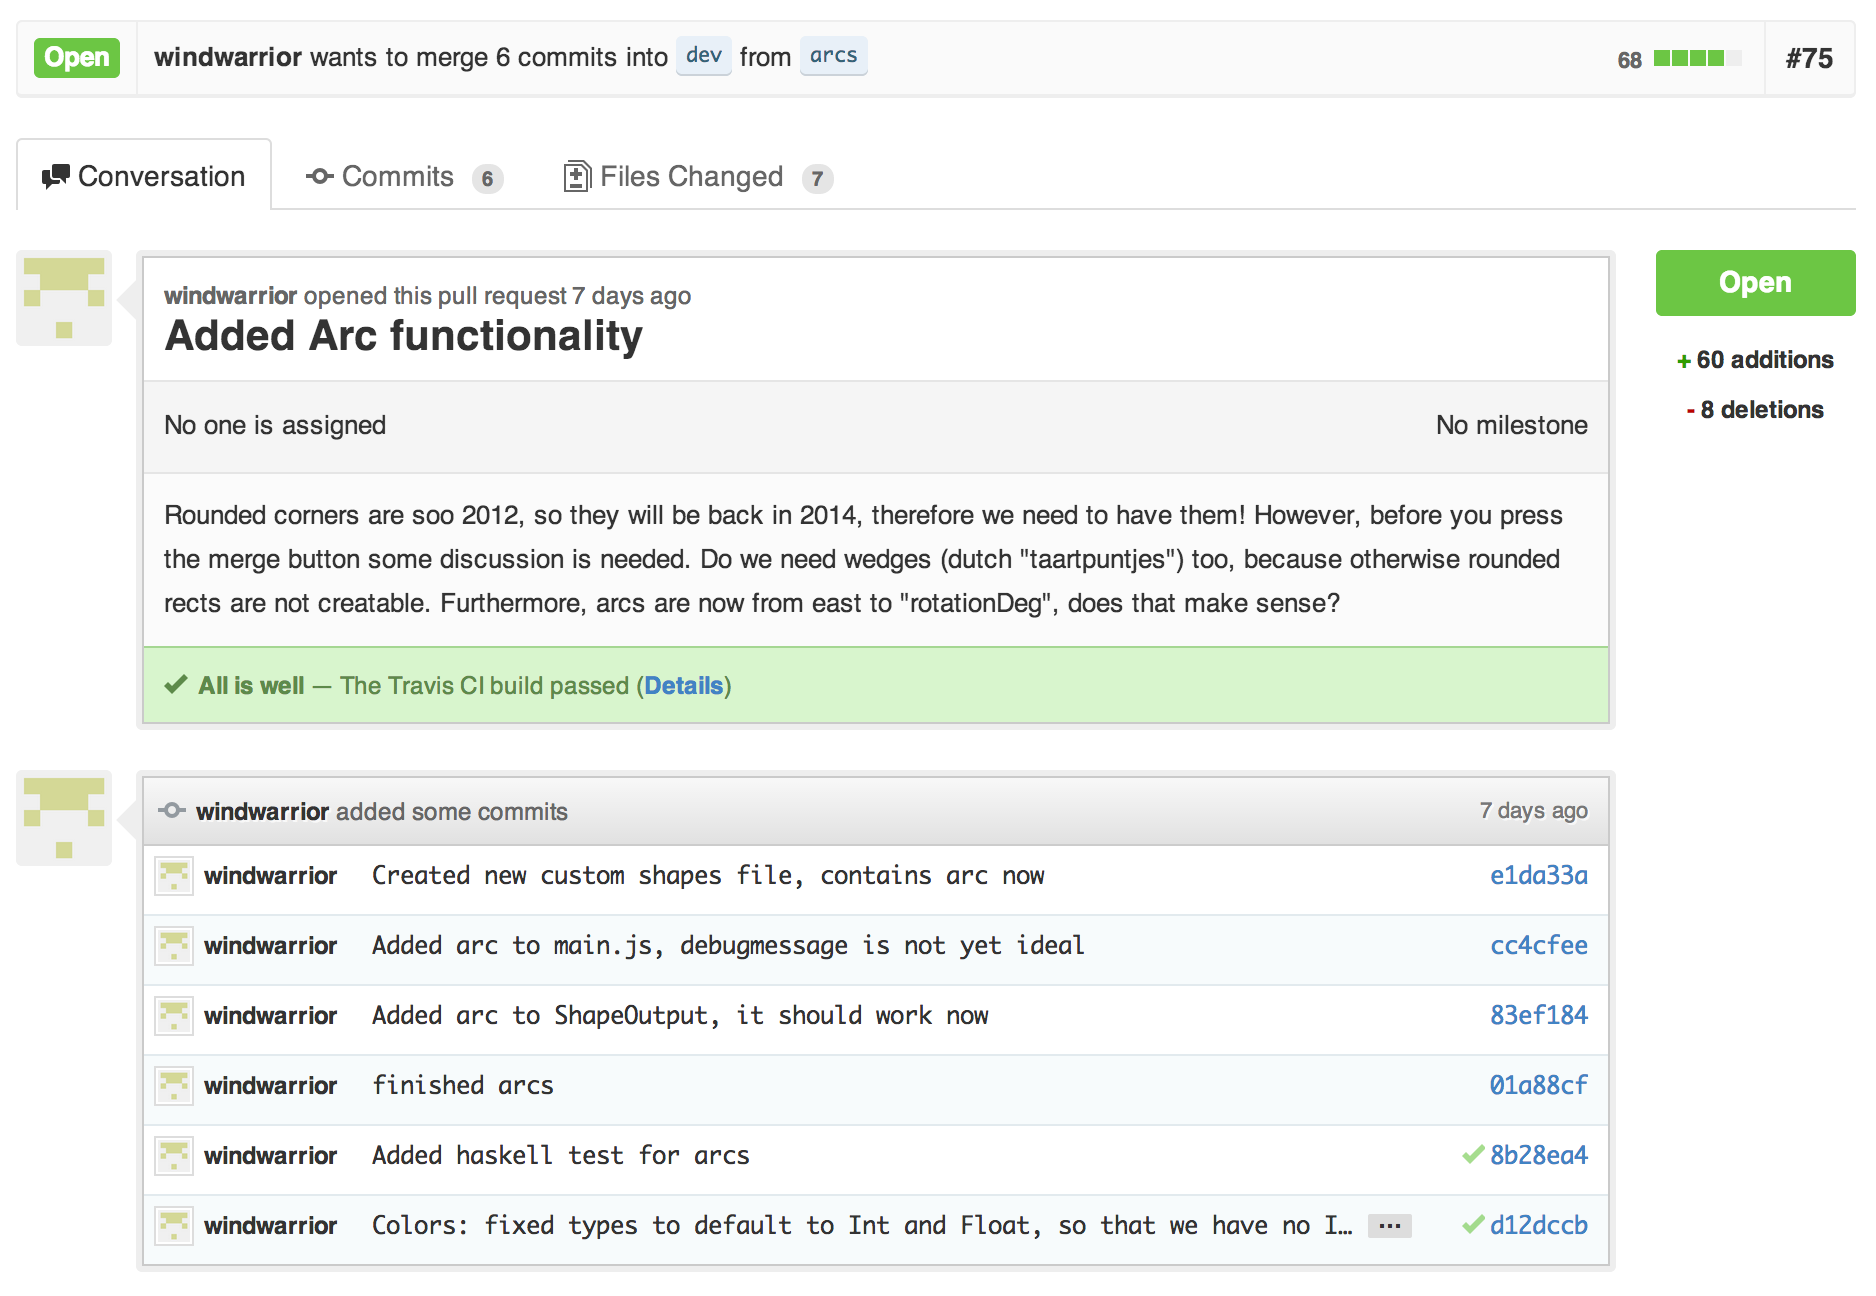
\includegraphics[keepaspectratio,width=\textwidth]{./images/pullrequest.png}
\caption{Pull Request \#75 Arcs geimplementeerd. – \url{https://github.com/CanvasHS/Canvas.hs/pull/75}}
\label{fig:pullrequest}
\end{center}
\end{figure}

Als een feature af is moet deze beoordeeld voordat deze gemergd kan worden naar de \inlinecode{dev} branch. Daarvoor wordt een \emph{pull request} aangemaakt. Deze \emph{pull request} bevat dan informatie over de wijzigingen tenopzichte van de versie die op de \inlinecode{dev} branch staat. Een beoordelaar kan de code lezen en deze goedkeuren. Op het moment dat de code goed wordt gekeurt komt een nieuwe versie met de nieuwe feature op de \inlinecode{dev} branch te staan.

Bij aanvang van het project was deze werkwijze voor veel teamleden nieuw. En daarom is het in het begin niet altijd juist toegepast. Maar naarmate het project vorderde is steeds vaker met succes gebruik gemaakt van het pull request principe. Dit zorgde er voor dat teamleden elkaars code controleerde en dat er minder bugs zaten in de versies op de \inlinecode{dev} branch.

\paragraph{Continuous integration} Om het beoordelen van code gemakkelijk te maken voor de ontwikkelaar en de beoordelaar is er gebruik gemaakt van de \emph{continuous integration} software \emph{Travis}. Deze software luistert naar nieuwe commits naar het centrale repository, als er een nieuwe commit gedaan is wordt er een virtuele machine opgestart die vervolgens middels een buildscript de versie van de software probeert te bouwen. Dit buildscript staat in de root directory van het repository.

Dit buildscript specificeert onder andere dat de software gebouwd moet worden met de Haskell compiler, maar ook dat alle geschreven tests uitgevoerd moeten worden. Mocht de compilatie of het uitvoeren van een van de tests niet geslaagd zijn is de build gefaald. Dit wordt dan vervolgens ook weergeven in het venster van de pull request. Als een beoordelaar ziet dat de build uit een pull request succesvol is, zoals bijvoorbeeld te zien bij \autoref{fig:pullrequest}, weet hij zeker dat de versie veilig is om te mergen.

Het buildscript voert naast de compilatie en de testen nog een paar andere commando's uit. Zo genereert het buildscript ook de documentatie en uploadet deze naar de Canvas.HS website—\url{http://canvashs.github.io}. Op de website kan de documentatie bekeken worden per build. Hierdoor hoeven ontwikkelaars zelf geen documentatie meer te genereren en hebben zij altijd, up to date, doorzoekbare documentatie.

\paragraph{Verbeteringen} Naast het integreren van documentatie zou het buildscript ook automatisch per versie de test coverage uit kunnen rekenen. Dit zou ontwikkelaars nog meer inzicht kunnen geven in de kwaliteit van de software en hoe deze voor– of achteruit gaat per versie.
